% !TEX root = ../main.tex
\documentclass[../main.tex]{subfiles}
\begin{document}
В этой главе рассмотрены варианты локальных угломерных навигационных систем, которые позволяют определять координаты и угловую ориентацию подвижных объектов.

%
% TODO: Привести в соответствие с первой статьей
%
%
\subsection{Локальная угломерная навигационная система первого типа}
Пусть три радиоориентира расположены в точках $M_1\left(x_1, y_1, z_1\right)$, $M_2\left(x_2, y_2, z_2\right)$ и $M_3\left(x_3, y_3, z_3\right)$ с заданными координатами и находятся не на одной прямой, а ФЦ БПА, размещенной на подвижном объекте находится в точке $M_0\left(x, y, z\right)$. В таком случае, эти четыре точки образуют в пространстве треугольную пирамиду, схематическое представление которой приведено на рисунке \ref{fig:tetrahedron:pic1}. Обозначим через $\ell_i$ длину бокового ребра $M_0M_i$, через $d_{ij}$ "--- длину ребра основания $M_iM_j$, а через $\alpha_{ij}$ "--- плоский угол $\angle M_iM_0M_j$ при вершине пирамиды. Пространственное положение подвижного объекта и радиоориентиров также будем определять с помощью радиус-векторов $\mathbf{r}_0 = \left(x, y, z\right)$ и $\mathbf{r}_i = \left(x_i, y_i, z_i\right)$ соответственно.

\begin{figure}[htbp]
    \begin{center}

    \fbox{\includegraphics[width=0.6\columnwidth]{3/tetrahedron/pic1}}

    \caption{Схема размещения в пространстве трех радиоориентиров и фазового центра БПА}
    \label{fig:tetrahedron:pic1}
    \end{center}
\end{figure}

Допустим, что в результате азимутально-угломестного радиопеленгования радиоориентиров с использованием БПА определены три пары азимутов $\alpha_{i}$ и углов места $\varepsilon_{i}$. Тогда в связаной системе координат БПА можно определить три единичных вектора $\mathbf{s}_{\text{св}i}$ направлений на каждый из радиоориентиров следующим образом:
\begin{equation}\label{eq:vecs}
    \mathbf{s}_{\text{св}i} = \left(\cos\alpha_i \cos\varepsilon_i, \sin\alpha_i\cos\varepsilon_i, \sin\varepsilon_i\right).
\end{equation}
С учетом (\ref{eq:vecs}), косинусы плоских углов $\alpha_{ij}$ равны
\begin{equation}
    \cos\alpha_{ij} = \left(\mathbf{s}_{\text{св}i}, \mathbf{s}_{\text{св}j}\right) =
    \cos\varepsilon_i \cos\varepsilon_j \cos\left(\alpha_i - \alpha_j\right) + \sin\varepsilon_i \sin\varepsilon_j
\end{equation}

С учетом вышеупомянутых значений, система уравнений для нахождения неизвестных значений длин $\ell_1$, $\ell_2$
и $\ell_3$ имеет следующий вид:
\begin{equation} \label{eq:system}
    \begin{cases}
    \ell_1^2 + \ell_2^2 - 2 \ell_1 \ell_2 \cos\alpha_{12} = d_{12}^2 \\
    \ell_1^2 + \ell_2^2 - 2 \ell_1 \ell_2 \cos\alpha_{12} = d_{12}^2 \\
    \ell_1^2 + \ell_2^2 - 2 \ell_1 \ell_2 \cos\alpha_{12} = d_{12}^2
    \end{cases}
\end{equation}

Как показали вычислительные эксперименты, система уравнений (\ref{eq:system}) относительно искомых значений $\ell_1$, $\ell_2$ и $\ell_3$ может иметь от одного до четырех решений в каждой из областей пространства, находящихся симметрично относительно плоскости расположения трех радиоориентиров. Структура этих решений и правила отбора истинного решения будут описаны далее. Предположим, что величины $\ell_1$, $\ell_2$ и $\ell_3$ найдены. В таком случае, для неизвестных $x$, $y$ и $z$ точки $M_0\left(x, y, z\right)$ расположения ФЦ БПА получим следующую систему из трех уравнений
\begin{equation}\label{eq:system_coordinates}
    \begin{cases}
        \left(x_1 - x\right)^2 + \left(y_1 - y\right)^2 + \left(z_1 - z\right)^2 = \ell_1^2 \\
        \left(x_2 - x\right)^2 + \left(y_2 - y\right)^2 + \left(z_2 - z\right)^2 = \ell_2^2 \\
        \left(x_3 - x\right)^2 + \left(y_3 - y\right)^2 + \left(z_3 - z\right)^2 = \ell_3^2
    \end{cases}
\end{equation}
Для решения системы уравнений (\ref{eq:system_coordinates}), вычтем из второго и третьего уравнений первое и перенесем члены, связанные с $z$ в правые части уравнений, в результате чего получим линейную относительно $x$ и $y$ систему уравнений:
\begin{equation}\label{eq:system_linear}
    \begin{cases}
        2x \left(x_1 - x_2\right) + 2 y \left(y_1 - y_2\right) =\ell_2^2 - \ell_1^2 + x_1^2 - x_2^2 + y_1^2 - y_2^2 + z_1^2 - z_2^2 - 2z\left(z_1 - z_2\right) \\
        2x \left(x_1 - x_3\right) + 2 y \left(y_1 - y_3\right) =\ell_3^2 - \ell_1^2 + x_1^2 - x_3^2 + y_1^2 - y_3^2 + z_1^2 - z_3^2 - 2z\left(z_1 - z_3\right)
    \end{cases}
\end{equation}
Выразив, используя правило Крамера, $x$ и $y$ через $z$ из системы (\ref{eq:system_linear}) и подставив полученные выражения в (\ref{eq:system_coordinates}), получим квадратное уравнение относительно $z$. Следует заметить, что определитель системы (\ref{eq:system_linear}) не равен нулю, так как точки $M_1$, $M_2$ и $M_3$ не лежат на одной прямой.

После нахождения координат точки $M_0$, можно определить три единичных вектора $\mathbf{s}_{\text{н}i}$ направлений на $i$-е радиоориентиры в соответствии с соотношением
\begin{equation*}
    \mathbf{s}_{\text{н}i} = \frac{\mathbf{r}_0 - \mathbf{r}_1}{|\mathbf{r}_0 - \mathbf{r}_1|}.
\end{equation*}

Определим квадратную матрицу $\mathbf{S}_{\text{н}}$ из векторов $\mathbf{s}_{\text{н}1}$, $\mathbf{s}_{\text{н}2}$ и $\mathbf{s}_{\text{н}3}$ в соответствии с
\begin{equation*}
    \mathbf{S}_{\text{н}} = \left(\mathbf{s}_{\text{н}1}^\text{т}, \mathbf{s}_{\text{н}2}^\text{т}, \mathbf{s}_{\text{н}3}^\text{т}\right).
\end{equation*}
Также определим квадратную матрицу $\mathbf{S}_{\text{св}}$ из векторов (\ref{eq:vecs}):
\begin{equation*}
    \mathbf{S}_{\text{св}} = \left(\mathbf{s}_{\text{св}1}^\text{т}, \mathbf{s}_{\text{св}2}^\text{т}, \mathbf{s}_{\text{св}3}^\text{т}\right).
\end{equation*}
В таком случае, квадратные матрицы $\mathbf{S}_{\text{н}}$ и $\mathbf{S}_{\text{св}}$ связаны соотношением
\begin{equation}\label{eq:matrix}
    \mathbf{S}_{\text{н}} = \mathbf{\xi}_{\text{св}}^{\text{н}} \times \mathbf{S}_{\text{св}},
\end{equation}
где $\mathbf{\xi}_{\text{св}}^{\text{н}}$ "--- квадратная матрица вращения при переходе от связной системы координат к нормальной земной системе координат. Таким образом, из (\ref{eq:matrix}) получим явное выражение для матрицы $\mathbf{\xi}_{\text{св}}^{\text{н}}$:
\begin{equation*}
    \mathbf{\xi}_{\text{св}}^{\text{н}} = \mathbf{S}_{\text{н}} \times \mathbf{S}_{\text{св}}^{-1},
\end{equation*}
где $\mathbf{S}_{\text{св}}^{-1}$ "--- обратная к $\mathbf{S}_{\text{св}}$ матрица. Углы курса $\psi$, крена $\mu$ и тангажа $\vartheta$ находятся из матрицы $\mathbf{\xi}_{\text{св}}^{\text{н}}$ стандартным образом.

%
%
% TODO: Привести в соответствие с окончательным вариантом второй статьи
%
%
\subsection{Случай локальной системы с НПУ}
В работе~\cite{antennas} рассматривалась локальная угломерная навигационная система (ЛУНС), состоящая из трех наземных радиоориентиров и воздушного объекта, оснащенного радиолокационным оборудованием, которое способно определять азимут и угол места каждого из наземных радиоориентиров. Авторами было показано, что определение пространственных координат и угловой ориентации воздушного объекта сводится к решению нелинейной системы уравнений следующего вида:
\begin{equation}\label{eq:luns_start}
  \begin{cases}
    \ell_1^2 + \ell_2^2 - 2 \ell_1 \ell_2 \cos \alpha_{12} = d_{12}^2 \\
    \ell_1^2 + \ell_3^2 - 2 \ell_1 \ell_3 \cos \alpha_{13} = d_{13}^2 \\
    \ell_2^2 + \ell_3^2 - 2 \ell_2 \ell_3 \cos \alpha_{23} = d_{23}^2 \\
  \end{cases},
\end{equation}
где $\ell_i$ "--- это расстояние от воздушного объекта до $i$-го радиоориентира, $d_{i,j}$ "--- расстояние между $i$-м и $j$-м наземным радиоориетиром, $\cos \alpha_{i,j}$ "--- плоский угол, образованный наземными ориентирами $i$ и $j$ и воздушным объектом. Из этой системы далее выводятся координаты и угловая ориентация воздушного объекта.

Система~(\ref{eq:luns_start}) может иметь несколько решений, что ведет к неоднозначности определения координат и угловой ориентации летательного аппарата. Поэтому, в статье~\cite{antennas} приводятся методики для расчета областей, где решение можно определить однозначно. Более того, решение системы~(\ref{eq:luns_start}) производится численно, что потенциально может привести к дополнительным ошибкам в определении пространственных параметров воздушного объекта. В связи с этим, далее предлагается еще один вариант ЛУНС, которая лишена вышеперечисленных недостатков ценой усложнения структуры системы.

Предлагается заменить один из пассивных радиоориентиров на наземный пункт управления (НПУ), оснащенный радиоориентиром. Требуется, чтобы НПУ мог определять азимут и угол места двух других радиоориентиров и воздушного объекта.

По аналогии с~\cite{antennas}, будем считать, что воздушный объект находится в точке $M_0\left(x, y, z\right)$, НПУ "--- в $M_1\left(x_1, y_1, z_1\right)$, а $i$-й РО "--- в точке $M_i\left(x_i, y_i, z_i \right)$, $i = 1,2$. Азимут и угол места радиоориентира $M_i$, полученные в результате радиопеленгования, обозначим через $\theta_i$ и $\beta_i$ соответственно (см. рис.~\ref{fig:systems:pic1}). Предполагается, что измерения этих углов проводятся в локальной системе координат НПУ, центр которой совпадает с координатами НПУ в НЗСК, а направления осей совпадают с НЗСК. В этой системе координат можно определить три единичных вектора направлений на радиоориентиры $M_0$, $M_2$ и $M_3$:
\begin{equation*}
  \mathbf{s}_{\text{лн}i} = \left(\cos\theta_i \cos\beta_i, \sin\theta_i\cos\beta_i, \sin\beta_i\right),
\end{equation*}
где $i = 0, 2, 3$. Тогда, косинусы углов $\alpha_{02} = \angle M_0 M_1 M_2$ и $\alpha_{03} = \angle M_0 M_1 M_3$ определяются как
\begin{align*}
  \cos\alpha_{02} = \left(\mathbf{s}_{\text{лн}0}, \mathbf{s}_{\text{лн}2}\right) =
  \cos\beta_0 \cos\beta_2 \cos\left(\theta_0 - \theta_2\right) + \sin\beta_0 \sin\beta_2, \\
  \cos\alpha_{03} = \left(\mathbf{s}_{\text{лн}0}, \mathbf{s}_{\text{лн}3}\right) =
  \cos\beta_0 \cos\beta_3 \cos\left(\theta_0 - \theta_3\right) + \sin\beta_0 \sin\beta_3.
\end{align*}

\begin{figure}[htbp]
  \begin{center}

  \fbox{\includegraphics[width=0.8\columnwidth]{3/systems/pic1}}

  \caption{Схемы размещения на местности БпЛА, НПУ и РО для реализации ЛУНС}
  \label{fig:systems:pic1}
  \end{center}
\end{figure}

По теореме синусов для треугольника $M_1 M_0 M_2$:
\begin{equation}\label{eq:luns_sin_1}
  \frac{\ell_2}{\sin\alpha_{02}} = \frac{d_{12}}{\sin\alpha_{12}} = \frac{\ell_1}{\sin\left(\alpha_{12} + \alpha_{02}\right)}.
\end{equation}
Аналогично для треугольника $M_1 M_0 M_3$:
\begin{equation}\label{eq:luns_sin_2}
    \frac{\ell_3}{\sin\alpha_{03}} = \frac{d_{13}}{\sin\alpha_{13}} = \frac{\ell_1}{\sin\left(\alpha_{13} + \alpha_{03}\right)}.
\end{equation}
Таким образом, из~(\ref{eq:luns_sin_1}):
\begin{equation*}
    \ell_2 = \frac{d_{12}\sin\alpha_{02}}{\sin\alpha_{12}}.
\end{equation*}
В то же время, из~(\ref{eq:luns_sin_2}):
\begin{equation*}
    \ell_3 = \frac{d_{13}\sin\alpha_{03}}{\sin\alpha_{13}}.
\end{equation*}
Длина $\ell_1$ может быть найдена из любого уравнения:
\begin{equation*}
    \ell_1 = \frac{d_{12}\sin\left(\alpha_{12} + \alpha_{02}\right)}{\sin\alpha_{12}} = \frac{d_{13}\sin\left(\alpha_{13} + \alpha_{03}\right)}{\sin\alpha_{13}}.
\end{equation*}
Далее пространственные координаты и угловая ориентация БПА определяется согласно~\cite{antennas}.

\subsection{Локальная система с уменьшенным количеством наземных РО}
В работе~\cite{antennas} было показано, что минимально возможное число наземных радиоориентиров, которое позволяет однозначно определять координаты и угловую ориентацию воздушного объекта, равно трем. Однако, это число можно уменьшить, если добавить в систему еще один подвижный объект с радиоориентиром и бортовой пеленгационной антенной.

Пусть подвижные объекты находятся в точках $M_1\left(x_1, y_1, z_1\right)$ и $M_2\left(x_2, y_2, z_2\right)$, а наземные ориентиры находятся в точках $M_3\left(x_3, y_3, z_3\right)$ и $M_4\left(x_4, y_4, z_4\right)$, а расстояние между ними равно $d_{34}$. В результате азимутально-угломестной радиопеленгации  $j$-го радиоориентира с борта $i$-го подвижного объекта ($i \ne j$), определяются углы азимута ($\alpha_{ij}$) и угла места ($\varepsilon_{ij}$) (см Рис.~\ref{fig:systems:pic2}). Пусть также $\ell_ij$ "--- расстояние между $i$-м и $j$-м радиоориентиром.

\begin{figure}[htbp]
    \begin{center}

    \fbox{\includegraphics[width=0.8\columnwidth]{3/systems/pic2}}

    \caption{Схемы размещения на местности БпЛА, НПУ и РО для реализации ЛУНС}
    \label{fig:systems:pic2}
    \end{center}
\end{figure}

Обозначим через $\mathbf{s}_{ij}$ единичные векторы, которые определяются следующим образом:
\begin{equation}
    \mathbf{s}_{ij} = \left(\cos\alpha_{ij} \cos\varepsilon_{ij}, \cos\alpha_{ij} \sin\varepsilon_{ij}, \sin\varepsilon_{ij}\right),
\end{equation}
где $i \ne j$, $i = 1,2$, $j = 1,2,3,4$. Также обозначим через $\gamma_{ij}$ углы, образованные воздушным объектом $M_1$ и радиоориентирами $i$ и $j$ ($i \ne j$), а через $\varphi_{ij}$ "--- углы, образованные воздушным объектом $M_2$ и теми же радиоориентирами. В таком случае, косинусы этих углов находятся по формулам:
\begin{align*}
    \cos\gamma_{ij} &= \left(\mathbf{s}_{1i}, \mathbf{s}_{1j}\right), i \ne j \ne 1, \\
    \cos\varphi_{ij} &= \left(\mathbf{s}_{2i}, \mathbf{s}_{2j}\right), i \ne j \ne 2.
\end{align*}

По теореме синусов для треугольника $M_1 M_2 M_3$:
\begin{equation}\label{eq:luns_2_sin_1}
    \frac{\ell_{12}}{\sin{M_1 M_3 M_2}} = \frac{\ell_{13}}{\sin{\varphi_{13}}} = \frac{\ell_{23}}{\sin{\gamma_{13}}}.
\end{equation}
Для треугольника $M_1 M_2 M_4$:
\begin{equation}\label{eq:luns_2_sin_2}
    \frac{\ell_{12}}{\sin{M_1 M_4 M_2}} = \frac{\ell_{14}}{\sin{\varphi_{14}}} = \frac{\ell_{24}}{\sin{\gamma_{24}}}.
\end{equation}
Из (\ref{eq:luns_2_sin_1}) и (\ref{eq:luns_2_sin_2}) получим отношения:
\begin{align}
     \frac{\ell_{23}}{\ell_{12}} = \frac{\sin{\gamma_{13}}}{\sin{M_1 M_3 M_2}}, \frac{\ell_{24}}{\ell_{12}} = \frac{\sin{\gamma_{14}}}{\sin{M_1 M_4 M_2}} \label{eq:luns_2_triag_1}\\
     \frac{\ell_{13}}{\ell_{12}} = \frac{\sin{\varphi_{13}}}{\sin{M_1 M_3 M_2}}, \frac{\ell_{14}}{\ell_{12}} = \frac{\sin{\varphi_{14}}}{\sin{M_1 M_4 M_2}} \label{eq:luns_2_triag_2}.
\end{align}
По теореме косинусов для треугольника $M_2 M_4 M_3$:
\begin{equation}\label{eq:luns_2_cos_1}
    \ell_{23}^2 + \ell_{24}^2 - 2 \ell_{23} \ell_{24} \cos\varphi_{34} = \ell_{34}^2.
\end{equation}
С учетом (\ref{eq:luns_2_triag_1}), (\ref{eq:luns_2_cos_1}) можно переписать в виде:
\begin{equation}
    \ell_{12}^2 k_1^2 + \ell_{12}^2 k_2^2 - 2 \ell_{12} \ell_{12} k_1 k_2 \cos\varphi_{34} = \ell_{34}^2,
\end{equation}
где $k_1 = \sin\gamma_{13} / \sin{M_1 M_3 M_2}$, а $k_2 = \sin\gamma_{14} / \sin{M_4 M_1 M_2}$.
Тогда $\ell_{12}$ выражается следующим образом:
\begin{equation}\label{eq:luns_2_ell_12}
    \ell_{12} = \frac{\ell_{34}}{\sqrt{k_1^2 + k_2 ^2 - 2 k_1 k_2 \cos\varphi_{34}}}.
\end{equation}
С учетом (\ref{eq:luns_2_ell_12}), из (\ref{eq:luns_2_triag_1}) и (\ref{eq:luns_2_triag_2}) находятся расстояния $\ell_{13}$, $\ell_{14}$, $\ell_{23}$ и $\ell_{24}$.

Для нахождения координат воздушного объекта $M_i$, введем радиус-вектор $\mathbf{r}_{i3}$, который определяется следующим образом:
\begin{equation}
    \mathbf{r}_{i3} = \mathbf{s}_{i3} \ell_{i3} = M_3 - M_i.
\end{equation}
Отсюда, координаты точки $M_i$ в НЗСК находятся из системы уравнений:
\begin{equation}
    \begin{cases}
        x_i = x_3 - \ell_{i3} \cos\alpha_{i3} \cos\varepsilon_{i3}, \\
        y_i = y_3 - \ell_{i3} \cos\alpha_{i3} \sin\varepsilon_{i3}, \\
        z_i = y_3 - \ell_{i3} \sin\varepsilon_{i3}.
    \end{cases}
\end{equation}
Следует заметить, что аналогичные рассуждения справедливы и относительно радиоориентира $M_4$. Совокупность расчетов координат относительно обоих наземных радиоориентиров позволяет ввести дополнительный контроль ошибок.

Отметим, что работоспособность такой конфигурации системы достигается только в случае, когда все четыре точки не лежат в одной плоскости. Это реализуется при расположении подвижных аппаратов $M_1$ и $M_2$ по разные стороны от прямой, образованной наземными радиоориентирами $M_3$ и $M_4$ (см. рис.~\ref{fig:systems:pic2}).

Матрица поворота и угловая ориентация каждого из объектов находится по алгоритму, представленному в работе~\cite{antennas}.

\subsection{Случай автономной системы}
Автономная угломерная радионавигационная система (АУНС) предназначена для определения координат и угловой ориентации в пространстве двух воздушных объектов, оснащенных высотомерами и бортовыми радиоориентирами с наземного пункта управления (НПУ), оснащенного радиоориентиром.
% Схема размещения на местности воздушных объектов и наземного пункта управления приведены на рис.~\ref{figure:pic3}.

Пусть радиоориентир НПУ расположен в точке $M_0$ с заранее известными координатами $M_0\left(x_0, y_0, z_0\right)$ в Балтийской системе координат (БСК), а воздушные объекты "--- в точках $M_1$ и $M_2$ с координатами $M_i\left(x_i, y_i, z_i\right)$, при этом $z_i$ совпадает с измерениями высотомера $h_i$. НПУ $M_0$ способен измерять радиопеленг $\theta_i$ и угол возвышения $\beta_i$ $i$-го воздушного объекта в БСК. Воздушные объект $M_n$ способен измерять азимут $\alpha_{ni}$ и угол места $\varepsilon_{ni}$ $i$-го радиоориентира (наземного или воздушного) в связанной системе координат БПА \cite{antennas}. Схема размещения с указанными величинами указана на рис.~\ref{fig:systems:pic3}. Пространственное положение радиоориентиров в БСК также можно охарактеризовать радиус-векторами $\mathbf{r}_i = \left(x_i, y_i, z_i\right)$, где $i = 1,2,3$.

\begin{figure}[htbp]
    \begin{center}

    \fbox{\includegraphics[width=0.8\columnwidth]{3/systems/pic3}}

    \caption{Схемы размещения на местности БпЛА, НПУ и РО для реализации АУНС}
    \label{fig:systems:pic3}
    \end{center}
\end{figure}

При детерминированном подходе для такой системы возможно однозначно определить координаты и угловую ориентацию воздушных объектов. Для этого нужно выполнить следующие ключевые шаги:
\begin{enumerate}
    \item Определить координаты воздушных объектов в БСК.
    \item Определить координаты радиоориентиров в связанной системе координат воздушного объекта $M_1$ ($\Sigma_{\text{св}1}$).
    \item Составить матрицу поворота системы координат $\Sigma_{\text{св}1}$ по алгоритму, представленному ниже.
    \item Определить углы поворота $\Sigma_{\text{св}1}$ по алгоритму, представленному в \cite{antennas}.
    \item Повторить предыдущие шаги для воздушного ориентира $M_2$.
\end{enumerate}

Первая часть алгоритма реализуется явно "--- совокупность данных с высотомеров воздушных объектов и углов $\theta_i$, $\beta_i$ позволяют определить координаты летательных аппаратов однозначно. Таким образом, координаты радиоориентира $M_1$ и $M_2$ определяются следующим отношениями:
\begin{equation}
    \begin{cases}
        x_1 = \rho_1 \cos\theta_1 \cos\beta_1 \\
        y_1 = \rho_1 \sin\theta_1 \cos\beta_1 \\
        z_1 = h_1 = \rho_1 \sin\beta_1 \\
        \rho_1 = ~^{z_1}/_{\sin\beta_1}
    \end{cases},
    \begin{cases}
        x_2 = \rho_2 \cos\theta_2 \cos\beta_2 \\
        y_2 = \rho_2 \sin\theta_2 \cos\beta_2 \\
        z_2 = h_2 = \rho_2 \sin\beta_2 \\
        \rho_2 = ~^{z_2}/_{\sin\beta_2}
    \end{cases}.
\end{equation}

Далее необходимо определить координаты радиоориентиров $M_0$ и $M_2$ в связанной системе координат воздушного объекта $M_1$:
\begin{equation}
    \begin{cases}
        x'_0 = \rho_{10} \cos\alpha_{10} \cos\varepsilon_{10} \\
        y'_0 = \rho_{10} \sin\alpha_{10} \cos\varepsilon_{10} \\
        z'_0 = z_1 - z_0 = \rho_{10} \sin\varepsilon_{10} \\
        \rho_{10} = |\mathbf{r}_1 - \mathbf{r}_0|
    \end{cases},
    \begin{cases}
        x'_2 = \rho_{12} \cos\alpha_{12} \cos\varepsilon_{12} \\
        y'_2 = \rho_{12} \sin\alpha_{12} \cos\varepsilon_{12} \\
        z'_2 = z_1 - z_2 = \rho_{12} \sin\varepsilon_{12} \\
        \rho_{12} = |\mathbf{r}_1 - \mathbf{r}_2|
    \end{cases},
\end{equation}
где $M_0'\left(x'_0, y'_0, z'_0\right)$ и $M_2'\left(x'_2, y'_2, z'_2\right)$
"--- координаты $M_0$ и $M_2$ в связанной СК $M_1$.

Для определения матрицы поворота системы координат $\Sigma_{\text{св}1}$, необходимо сначала ввести радиус-вектора $\mathbf{r}'_0 = \left(x'_0, y'_0, z'_0\right)$ и $\mathbf{r}'_2 = \left(x'_2, y'_2, z'_2\right)$, которые определяют положения радиоориентиров $M_0$ и $M_2$ в связанной системе координат $M_1$. Далее, зададим единичные векторы $\mathbf{s}'_1$, $\mathbf{s}'_2$ и $\mathbf{s}'_3$ следующим образом:
\begin{equation}\label{eq:vec_1_local}
    \begin{split}
    \mathbf{s}'_1 = \left(s'_{1x}, s'_{1y}, s'_{1z}\right) = &\left(\cos\alpha_{10} \cos\varepsilon_{10}, \sin\alpha_{10}\cos\varepsilon_{10}, \sin\varepsilon_{10}\right),\\
    \mathbf{s}'_2 = \left(s'_{2x}, s'_{2y}, s'_{2z}\right) = &\left(\cos\alpha_{12} \cos\varepsilon_{12}, \sin\alpha_{12}\cos\varepsilon_{12}, \sin\varepsilon_{12}\right),\\
    \mathbf{s}'_3 = \mathbf{s}'_1 \times \mathbf{s}'_2 = \left(s'_{3x}, s'_{3y}, s'_{3z}\right) = &\left(\sin\alpha_{12}\cos\varepsilon_{12}\sin\varepsilon_{10} - \sin\alpha_{12}\sin\alpha_{10}\cos\varepsilon_{10},\right.\\
    &\ \sin\alpha_{10}\cos\varepsilon_{10}\sin\varepsilon_{12} - \cos\alpha_{10}\cos\varepsilon_{12}\sin\varepsilon_{10},\\
    &\ \left.\sin\left(\alpha_{10} - \alpha_{12}\right)\cos\varepsilon_{10}\cos\varepsilon_{12}\right).
    \end{split}
\end{equation}
Те же вектора в балтийской системе координат:
\begin{equation}\label{eq:vec_1_bsk}
    \begin{split}
        \mathbf{s}_{01} &= \left(s_{01x}, s_{01y}, s_{01z}\right) = \frac{\mathbf{r}_0 - \mathbf{r}_1}{|\mathbf{r}_0 - \mathbf{r}_1|},\\
        \mathbf{s}_{21} &= \left(s_{21x}, s_{21y}, s_{21z}\right) = \frac{\mathbf{r}_2 - \mathbf{r}_1}{|\mathbf{r}_2 - \mathbf{r}_1|},\\
        \mathbf{n}_1 &= \left(n_{1x}, n_{1y}, n_{1z}\right) = \mathbf{s}_{01} \times \mathbf{s}_{21}.\\
    \end{split}
\end{equation}
Определим квадратную матрицу $\mathbf{S}$ размера $3 \times 3$ координат трех полученных по формуле (\ref{eq:vec_1_bsk}) единичных векторов $\mathbf{s}_{01}$, $\mathbf{s}_{21}$ и $\mathbf{n}_{1}$, записав в столбцы, в соответствии с отношением:
\begin{equation}\label{eq:vec_1_bsk_matrix}
    \mathbf{S}_1 =
    \left(
        \begin{matrix}
            s_{01x} & s_{01y} & s_{01z} \\
            s_{21x} & s_{21y} & s_{21z} \\
            n_{1x} & n_{1y} & n_{1z}
        \end{matrix}
    \right).
\end{equation}
По аналогии с (\ref{eq:vec_1_bsk_matrix}) определим квадратную матрицу $\mathbf{S}'$ размера $3 \times 3$ координат трех полученных по формуле (\ref{eq:vec_1_local}):
\begin{equation}\label{eq:vec_1_local_matrix}
    \mathbf{S}' =
    \left(
        \begin{matrix}
            s'_{1x} & s'_{1y} & s'_{1z} \\
            s'_{2x} & s'_{2y} & s'_{2z} \\
            s'_{3x} & s'_{3y} & s'_{3z}
        \end{matrix}
    \right).
\end{equation}
Отсюда получим следующее преобразование координат:
\begin{equation*}
    \mathbf{R_1} \times \mathbf{S}_1 = \mathbf{S}'
\end{equation*}

В таком случае, матрицу поворота связанной системы координат $\Sigma_{\text{св}1}$ можно найти следующим образом:
\begin{equation}
    \mathbf{R_1} = \mathbf{S}' \times \mathbf{S}_1^{-1}
\end{equation}

По аналогии можно получить матрицу поворота $\mathbf{R}_2$ связанной системы координат $M_2$. Вводятся радиус-вектора $\mathbf{r}''_0 = \left(x''_0, y''_0, z''_0\right)$,
$\mathbf{r}''_1 = \left(x''_1, y''_1, z''_1\right)$, по ним же определяются единичные вектора
$\mathbf{s}''_1$, $\mathbf{s}''_2$ и $\mathbf{s}''_3$:
\begin{equation}\label{eq:vec_2_local}
    \begin{split}
    \mathbf{s}''_1 = \left(s''_{1x}, s''_{1y}, s''_{1z}\right) =  &\left(\cos\alpha_{20} \cos\varepsilon_{20}, \sin\alpha_{20}\cos\varepsilon_{20}, \sin\varepsilon_{20}\right),\\
    \mathbf{s}''_2 = \left(s''_{2x}, s''_{2y}, s''_{2z}\right) = &\left(\cos\alpha_{21} \cos\varepsilon_{21}, \sin\alpha_{21}\cos\varepsilon_{21}, \sin\varepsilon_{21}\right),\\
    \mathbf{s}''_3 = \mathbf{s}''_1 \times \mathbf{s}''_2 = \left(s''_{3x}, s''_{3y}, s''_{3z}\right) =  &\left(\sin\alpha_{21}\cos\varepsilon_{21}\sin\varepsilon_{20} - \sin\alpha_{21}\sin\alpha_{20}\cos\varepsilon_{20},\right.\\
    &\ \sin\alpha_{20}\cos\varepsilon_{20}\sin\varepsilon_{21} - \cos\alpha_{20}\cos\varepsilon_{21}\sin\varepsilon_{20},\\
    &\ \left.\sin\left(\alpha_{20} - \alpha_{21}\right)\cos\varepsilon_{20}\cos\varepsilon_{21}\right).
    \end{split}
\end{equation}
В балтийской системе координат:
\begin{equation}\label{eq:vec_2_bsk}
    \begin{split}
        \mathbf{s}_{02} &= \left(s_{01x}, s_{01y}, s_{01z}\right) = \frac{\mathbf{r}_0 - \mathbf{r}_2}{|\mathbf{r}_0 - \mathbf{r}_1|},\\
        \mathbf{s}_{21} &= \left(s_{21x}, s_{21y}, s_{21z}\right) = \frac{\mathbf{r}_2 - \mathbf{r}_1}{|\mathbf{r}_2 - \mathbf{r}_1|},\\
        \mathbf{n}_1 &= \left(n_{1x}, n_{1y}, n_{1z}\right) = \mathbf{s}_{02} \times \mathbf{s}_{21}.\\
    \end{split}
\end{equation}
Определим квадратные матрицы $\mathbf{S}_2$ и $\mathbf{S}''$ размера $3 \times 3$ по аналогии с (\ref{eq:vec_1_bsk_matrix}) и (\ref{eq:vec_1_local_matrix}):
\begin{equation}\label{eq:vec_1_bsk_matrix}
    \mathbf{S}_2 =
    \left(
        \begin{matrix}
            s_{01x} & s_{01y} & s_{01z} \\
            s_{21x} & s_{21y} & s_{21z} \\
            n_{1x} & n_{1y} & n_{1z}
        \end{matrix}
    \right),
    \mathbf{S}'' =
    \left(
        \begin{matrix}
            s''_{1x} & s''_{1y} & s''_{1z} \\
            s''_{2x} & s''_{2y} & s''_{2z} \\
            s''_{3x} & s''_{3y} & s''_{3z}
        \end{matrix}
    \right).
\end{equation}
Отсюда, матрица поворота определяется следующим образом:
\begin{equation}
    \mathbf{R_2} = \mathbf{S}'' \times \mathbf{S}_2^{-1}
\end{equation}

Углы курса $\psi_1$, $\psi_2$, крена $\mu_1$, $\mu_2$ и тангажа $\vartheta_1$, $\vartheta_2$ находятся
из матриц $\mathbf{R}_1$ и $\mathbf{R}_2$ в соответствии с~\cite{antennas}.

%
%
% TODO: Привести в соответствие с финальной версией статьи
%
\subsection{Влияние подстилающей поверхности на точность измерений}
Рассматривается трехэлементная вертикальная система датчиков с расстоянием $\Delta h$  между соседними элементами. Предполагается, что принимаемый сигнал формируется как суперпозиция двух плоских электромагнитных волн одинаковой частоты. Первая из них, приходящая от регистрируемого источника, имеет амплитуду $E_0$ и фазу на среднем элементе $\varphi _0$. Вторая представляет отраженную от поверхности Земли волну с амплитудой $E_1$ и фазой на среднем элементе $\varphi _1$. Соответствующие комплексные компоненты принимаемого сигнала задаются формулами
\begin{equation*}
  \dot{E}_0=E_0 e^{i\varphi _0}, \; \dot{E}_1=E_1 e^{i\varphi _1}.
\end{equation*}

Пусть $\beta_0$ "--- угол отклонения волны источника от горизонта (считаем, что источник находится выше датчиков), $\beta_1$ "--- угол отклонения отраженной волны от горизонта (отражение происходит ниже датчиков), $\lambda$ "--- длина волны приходящего сигнала. Введем следующие обозначения:
\begin{equation}\label{eq:w_0_w_1}
  \omega_0= \frac{2\pi}{\lambda} \Delta h \sin \beta_0, \;
  \omega_1= \frac{2\pi}{\lambda} \Delta h \sin \beta_1.
\end{equation}
Тогда для комплексных сигналов $\dot{z}_0, \dot{z}_{\hbox{н}}, \dot{z}_{\hbox{в}}$, регистрируемых на среднем, нижнем и верхнем датчиках, соответственно, справедливы следующие соотношения
\begin{equation} \label{eq:0_down_up}
  \begin{cases}
    \dot{z}_0  = \dot{E}_0 + \dot{E}_1 \\
    \dot{z}_\text{н} = \dot{E}_0 e^{-i\omega_0} + \dot{E}_1 e^{i\omega_1} \\
    \dot{z}_\text{в} = \dot{E}_0 e^{i\omega_0} + \dot{E}_1 e^{-i\omega_1}
  \end{cases}
\end{equation}
Требуется по заданным величинам $\dot{z}_0, \dot{z}_{\hbox{н}}, \dot{z}_{\hbox{в}}$ определить угол $\beta_0$.

\begin{figure}[htbp]
  \begin{center}

  \fbox{\includegraphics[width=0.9\columnwidth]{3/surface/pic1}}

  \caption{Геометрия расчетной модели эквидистантной трехэлементной антенной решетки из соосных вертикальных вибраторных антенн}
  \label{figure:surface:pic1}
  \end{center}
\end{figure}

Система \eqref{eq:0_down_up} содержит три комплексных уравнения относительно шести неизвестных вещественных величин $\beta_0$, $\beta_1$, $E_0$, $E_1$, $\varphi_0$, $\varphi_1$ и является нелинейной. Выбор данной модели обусловлен тем, что удается аналитически исключить из этой системы все переменные кроме $\omega_0$, которая включает, согласно \eqref{eq:w_0_w_1}, интересующую нас величину $\beta_0$.

\subsubsection{Решение системы}
Для исключения $\dot{E}_0$ умножим второе уравнение \eqref{eq:0_down_up} на $e^{i\omega_0}$, третье уравнение "--- на $e^{-i\omega_0}$. Тогда
\begin{equation*}
  \begin{cases}
    \dot{z}_0 = \dot{E}_0 + \dot{E}_1 \\
    \dot{z}_\text{н} e^{ i\omega_0} = \dot{E}_0 + \dot{E}_1 e^{ i \left(\omega_1 + \omega_0 \right)} \\
    \dot{z}_\text{в} e^{-i\omega_0} = \dot{E}_0 + \dot{E}_1 e^{-i \left(\omega_1 + \omega_0\right)}
  \end{cases}
\end{equation*}
Вычитая первое уравнение полученной системы из второго и третьего уравнений, приходим к системе двух комплексных уравнений
\begin{equation*}
  \begin{cases}
    \dot{z}_\text{н} e^{ i\omega_0} - \dot{z}_0 = \dot{E}_1 \left( e^{ i\left(\omega_1 + \omega_0 \right)} - 1\right) \\
    \dot{z}_\text{в} e^{-i\omega_0} - \dot{z}_0 = \dot{E}_1 \left( e^{-i\left(\omega_1 + \omega_0 \right)} - 1 \right)
  \end{cases}
\end{equation*}
Для исключения $\dot{E}_1$ домножим второе уравнение на $e^{i \left(\omega_1 + \omega_0 \right)}$ и сложим с первым:
\begin{equation*}
  \dot{z}_\text{н} e^{i\omega_0} - \dot{z}_0 + \left(\dot{z}_\text{в} e^{-i\omega_0} - \dot{z}_0 \right) e^{i \left(\omega_1 + \omega_0 \right)} = 0.
\end{equation*}
Таким образом,
\begin{equation*}
  \dot{z}_\text{н} e^{i\omega_0} - \dot{z}_0 = -\left(\dot{z}_\text{в} e^{-i\omega_0} - \dot{z}_0 \right) e^{i\left(\omega_1+\omega_0\right)}.
\end{equation*}
Осталось исключить $\omega_1$, для чего достаточно взять модуль от левой и правой частей последнего равенства
\begin{equation} \label{eq:w_0}
  \left|\dot{z}_\text{н} e^{i\omega_0} - \dot{z}_0 \right| = \left|\dot{z}_\text{в} e^{-i\omega_0} - \dot{z}_0\right|.
\end{equation}
Аналогичное соотношение получается и для $\omega_1$:
\begin{equation} \label{eq:w_1}
  \left|\dot{z}_\text{н} e^{-i\omega_1} - \dot{z}_0 \right| = \left|\dot{z}_\text{в} e^{i\omega_1} - \dot{z}_0 \right|.
\end{equation}

\subsubsection{Анализ разрешимости уравнения относительно $\beta_0$}

Запишем уравнение \eqref{eq:w_0} в следующем виде
\begin{equation*}
  \left|\dot{z}_\text{н} e^{ i \omega_0} - \dot{z}_0 \right|^2 =
  \left|\dot{z}_\text{в} e^{-i \omega_0} - \dot{z}_0 \right|^2.
\end{equation*}
Воспользовавшись тем, что $\left|\dot{z}\right|^2= \dot{z} \dot{z}^*$, где $\dot{z}^*$ означает комплексное сопряжение, придем к равенству
\begin{equation*}
  \left(\dot{z}_\text{н} e^{ i\omega_0} - \dot{z}_0 \right) \left(\dot{z}_\text{н} e^{ i\omega_0} - \dot{z}_0 \right)^* = \left(\dot{z}_\text{в} e^{-i\omega_0} - \dot{z}_0 \right) \left(\dot{z}_\text{в} e^{-i\omega_0} - \dot{z}_0 \right)^*.
\end{equation*}
Раскрывая скобки, получим
\begin{equation*}
  \left|\dot{z}_\text{н}\right|^2 - \dot{z}_\text{н} \dot{z}_{0}^* e^{ i\omega_0} \dot{z}_\text{н}^* \dot{z}_{0} e^{-i\omega_0} + \left|\dot{z}_{0}\right|^2 =
  \left|\dot{z}_\text{в} \right|^2 - \dot{z}_\text{в} \dot{z}_{0}^* e^{-i\omega_0} - \dot{z}_\text{в}^* \dot{z}_{0} e^{i\omega_0} + \left|\dot{z}_{0}\right|^2.
\end{equation*}
Перегруппируем слагаемые:
\begin{equation*}
  \left(\dot{z}_\text{в}^* \dot{z}_{0} - \dot{z}_\text{н} \dot{z}_{0}^* \right) e^{ i\omega_0} + \left(\dot{z}_\text{в} \dot{z}_{0}^* - \dot{z}_\text{н}^* \dot{z}_{0} \right) e^{-i\omega_0} = \left|\dot{z}_\text{в}\right|^2 - \left|\dot{z}_\text{н}\right|^2.
\end{equation*}
Обозначим
\begin{equation} \label{eq:u_v}
  \dot{z}_\text{в}^* \dot{z}_{0} - \dot{z}_\text{н} \dot{z}_{0}^* = u - iv.
\end{equation}
Тогда $\dot{z}_\text{в} \dot{z}_{0}^* - \dot{z}_\text{н}^* \dot{z}_{0} = u + iv$, и
\begin{equation*}
  \left(u - iv\right) \left(\cos\omega_0 + i \sin\omega_0\right) + \left(u + iv\right) \left(\cos\omega_0 - i \sin\omega_0\right) = \left|\dot{z}_\text{в}\right|^2 - \left|\dot{z}_\text{н}\right|^2.
\end{equation*}
Соответственно,
\begin{equation} \label{eq:u_v_omega_0}
  u \cos\omega_0 + v \sin\omega_0 =
  \frac{ \left|\dot{z}_\text{в}\right|^2 - \left|\dot{z}_\text{н}\right|^2} {2}=c.
\end{equation}

Условие разрешимости уравнения \eqref{eq:u_v_omega_0} может быть записано в следующем виде
\begin{equation} \label{eq:c_good}
  u^2 + v^2 \geq c^2.
\end{equation}
Для решения \eqref{eq:u_v_omega_0} перейдем к половинному углу
\begin{equation*}
  u \left( \cos^2\frac{\omega_0}{2} - \sin^2\frac{\omega_0}{2} \right) + 2v \sin\frac{\omega_0}{2} \cos\frac{\omega_0}{2} =
  c \left(\cos^2\frac{\omega_0}{2} + \sin^2\frac{\omega_0}{2} \right)
\end{equation*}
и перегруппируем слагаемые
\begin{equation*}
  \left(u - c\right) \cos^2\frac{\omega_0}{2} + 2v \sin\frac{\omega_0}{2} \cos\frac{\omega_0}{2} - \left(u + c\right) \sin^2\frac{\omega_0}{2} = 0.
\end{equation*}
Если $\left|u - c\right| > \left|u + c\right|$, то делим данное уравнение на $\sin^2 \sfrac{\omega_0}{2}$, в противном случае делим на $\cos^2 \sfrac{\omega_0}{2}$. В первом случае получается квадратное уравнение относительно $\ctg \sfrac{\omega_0}{2}$:
\begin{equation*}
    \left(u - c\right) \ctg^2 \frac{\omega_0}{2} + 2v \ctg\frac{\omega_0}{2} - \left(u + c\right) = 0,
\end{equation*}
во втором случае "--- относительно $\tg \frac{\omega_0}{2}$:
\begin{equation*}
    \left(u + c\right) \tg^2 \frac{\omega_0}{2} - 2v \tg \frac{\omega_0}{2} - \left(u - c\right) = 0.
\end{equation*}
Дискриминант для обоих уравнений равен $4\left(u^2 + v^2 - c^2\right)$ и в силу \eqref{eq:c_good} неотрицателен.

Поскольку $\beta_0 > \ang{0}$, то и $\omega_0 > 0$, а из ограничений сверху на параметры рассматриваемой модели $\beta_0 \leq \ang{15}$ и $ \Delta h^{}/\lambda \leq 3.5$ следует, что $\omega_0 < 2 \pi $. Соответственно, $0 < \rfrac{\omega_0}{2} < \pi$. Пусть, например, $t_1$, $t_2$ "--- корни квадратного уравнения относительно $\tg \rfrac{\omega_0}{2}$. Если оба корня положительные, то выбираем меньший из них $t_1$. Тогда
\begin{equation*}
  \omega_0 = 2 \arctg t_1, \; \beta_0 = \arcsin \frac{\omega_0 \lambda} {2\pi \Delta h}.
\end{equation*}
Если корни разных знаков, то выбираем положительный. Если оба корня отрицательные, то выбираем больший по модулю $t_1$ и полагаем $\omega_0 = 2\left( \arctg t_1 + \pi\right)$. В случае кратного корня делаем то же самое, только не требуется выбирать один из двух корней.
Несколько проще случай уравнения относительно $\ctg\rfrac{\omega_0}{2}$. Из двух возможных значений корней выбирается больший.

Возможен и численный метод решения уравнения \eqref{eq:u_v_omega_0}, например, метод половинного деления. В качестве начального отрезка для $\beta_0$ выбирается отрезок $[\ang{0}, \ang{15}]$, для середины отрезка вычисляется  $\omega_0$ по формуле \eqref{eq:w_0_w_1} и отрезок сужается вдвое. Количество итераций определяется поставленной точностью вычислений. Подводя итог, можно сказать, что для решения исходной задачи определения угла $\beta_0$ надо по заданным входным данным $\dot{z}_\text{в}$, $\dot{z}_{0}$, $\dot{z}_\text{н}$ определить согласно формуле \eqref{eq:u_v} вспомогательные величины $u$, $v$ и решить аналитически или численно тригонометрическое уравнение \eqref{eq:u_v_omega_0}.

\begin{figure}[htp]
  \centering
  \subfloat[\textit{а)}]{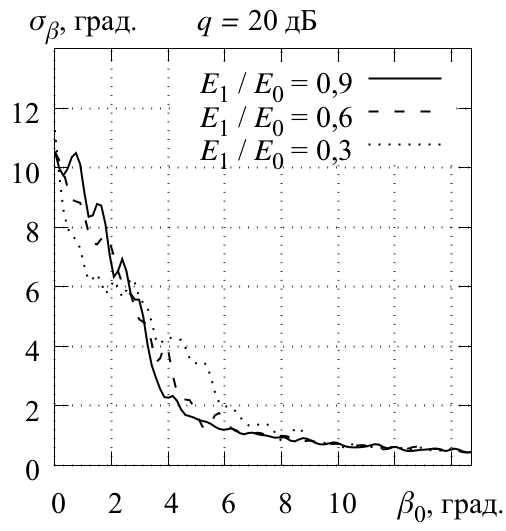
\includegraphics[width=0.3\linewidth]{3/surface/pic2_a}}
  \subfloat[\textit{б)}]{\includegraphics[width=0.3\linewidth]{3/surface/pic2_b}}
  \subfloat[\textit{в)}]{\includegraphics[width=0.3\linewidth]{3/surface/pic2_c}}
  \\
  \subfloat[\textit{г)}]{\includegraphics[width=0.3\linewidth]{3/surface/pic2_d}}
  \subfloat[\textit{д)}]{\includegraphics[width=0.3\linewidth]{3/surface/pic2_e}}
  \subfloat[\textit{е)}]{\includegraphics[width=0.3\linewidth]{3/surface/pic2_f}}
  
  \caption{Графики угловых зависимостей случайных (\textit{а}, \textit{б}, \textit{в}) и методических (\textit{г}, \textit{д}, \textit{е}) СКО определения угла при различных значениях параметров принятого сигнала: амплитуды (\textit{а}, \textit{г}), угла приема отраженной волны (\textit{б}, \textit{д}) и разности фаз принятых сигналов (\textit{в}, \textit{е}).}
  \label{fig:surface:pic2} 
\end{figure}

\subsubsection{Статистический анализ погрешности}

Наличие явного метода решения системы существенно облегчает анализ погрешности. Стандартным образом возмущаются входные данные $\dot{z}_\text{в}$, $\dot{z}_{о}$ и $\dot{z}_\text{н}$ с заданным отношением сигнал/шум (ОСШ) $q$, решается полученная система и вычисляется среднеквадратичная ошибка $\sigma_\beta$ определения угла $\beta_0$.

Возмущения исходных значений сигналов на каждой из антенн производилось путем добавления к ним некоторой случайной величины, распределенной по нормальному закону с нулевым математическим ожиданием и дисперсией, соответствующей заданному ОСШ. Устойчивость предложенного метода определения угла $\beta_0$ оценивалась при значении ОСШ $q = \SI{20}{\deciBells}$. Также при оценке рассматривался идеальный случай, в котором влияние шума пренебрежимо мало, т.е. ОСШ $q = \SI{100}{\deciBells}$. На Рис.~\ref{fig:surface:pic2} приведены графики зависимостей СКО $\sigma_\beta$ от определяемого угла $\beta_0$.

\begin{figure}[hpb]
  \centering
  \subfloat[\textit{а)}]{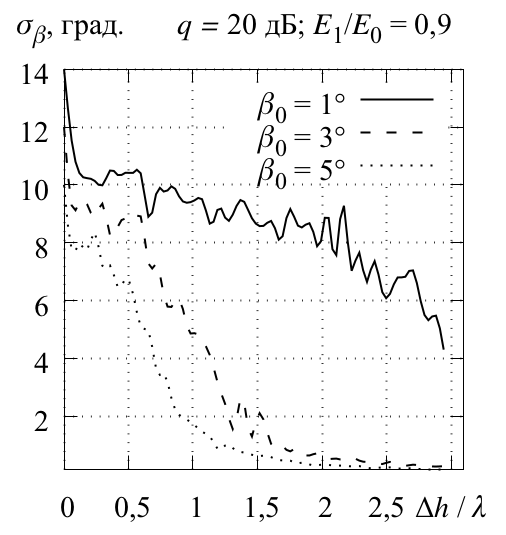
\includegraphics[width=0.3\linewidth]{3/surface/pic3_a}}
  \subfloat[\textit{б)}]{\includegraphics[width=0.3\linewidth]{3/surface/pic3_b}}
  \subfloat[\textit{в)}]{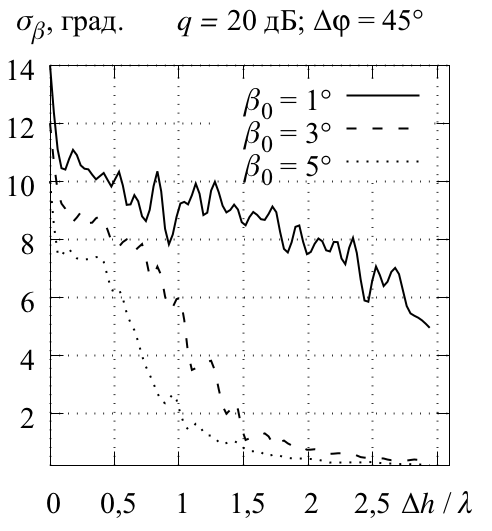
\includegraphics[width=0.3\linewidth]{3/surface/pic3_c}}
  \\
  \subfloat[\textit{г)}]{\includegraphics[width=0.3\linewidth]{3/surface/pic3_d}}
  \subfloat[\textit{д)}]{\includegraphics[width=0.3\linewidth]{3/surface/pic3_e}}
  \subfloat[\textit{е)}]{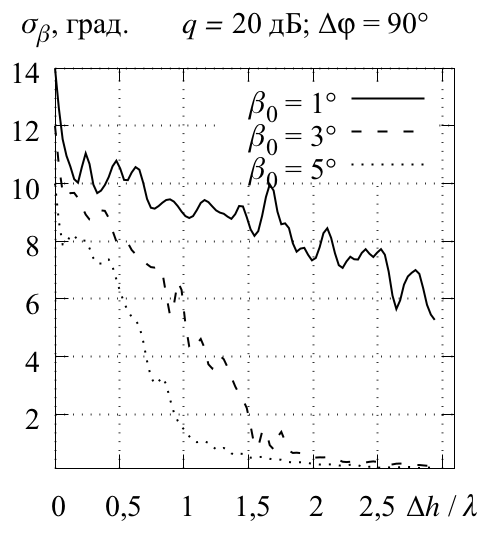
\includegraphics[width=0.3\linewidth]{3/surface/pic3_f}}

  \caption{Графики частотных зависимостей случайных СКО определения угла при различных значениях параметров принятого сигнала: амплитуды (\textit{а}, \textit{г}), угла приема отраженной волны (\textit{б}, \textit{д}) и разности фаз принятых сигналов (\textit{в}, \textit{е}).}
  \label{fig:surface:pic3}
\end{figure}

Также была произведена оценка зависимости СКО от уровня взаимного влияния между антеннами $\Delta h^{}/\lambda$. На Рис.~\ref{fig:surface:pic3} приведены графики этих зависимостей при различных значениях углов $\beta_0$ и значений параметров принятых сигналов.

С помощью моделирования было так же выяснено, что при увеличении ОСШ кривая угловых зависимостей СКО приобретает ярко выраженный L-образный характер, т.е. погрешность резко убывает при определенном значении определяемого угла $\beta_0$. Рис.~\ref{fig:surface:pic4} показывает характер этой зависимости при ОСШ $q = \SI{30}{\deciBells}$.

\begin{figure}[hpb]
  \centering
  \subfloat[\textit{а)}]{\includegraphics[width=0.3\linewidth]{3/surface/pic4_a}}
  \subfloat[\textit{б)}]{\includegraphics[width=0.3\linewidth]{3/surface/pic4_b}}
  \subfloat[\textit{в)}]{\includegraphics[width=0.3\linewidth]{3/surface/pic4_c}}

  \caption{Графики угловых зависимостей случайных СКО определения угла при различных значениях параметров принятого сигнала: амплитуды (\textit{а}), угла приема отраженной волны (\textit{б}) и разности фаз принятых сигналов (\textit{в})}
  \label{fig:surface:pic4}
\end{figure}

Главное отличие от модели, предложенной в [ВГМНП], состоит в том, что система содержит шесть неизвестных вещественных переменных, а не пять, и поэтому не является переопределенной. Соответственно, нет областей изменения параметров, в которых система несовместна. Сложности, как и следовало ожидать, начинаются при стремлении $\beta_0$ к нулю "--- в этом случае все три коэффициента $u$, $v$ и $c$ уравнения \eqref{eq:u_v_omega_0} становятся малыми, и преобразования, связанные с делением на эти величины, являются неустойчивыми.

Из приведенных в статье графиков среднеквадратичных погрешностей (рис. 2 и 3) можно сделать следующий вывод: если $\beta_0$ имеет величину порядка $\ang{1}$ "--- $\ang{3}$, то погрешность становится больше самой определяемой величины, т.е. вычисления с практической точки зрения бесполезны. Существенным оказывается и соотношение углов $\beta_0$ и $\beta_1$. С увеличением разности между ними растет и погрешность. Большая разность между этими углами возможна в том случае, когда объект пеленгации находится слишком близко к датчикам. Достаточно важным параметром является разность фаз $\Delta \varphi$ – если пришедшие сигналы приходят в фазе или противофазе, то предложенная модель оказывается неэффективной. Это объясняется тем, что величины $\dot{z}_\text{в}$ и $\dot{z}_\text{н}$ становятся слишком близки друг к другу и критерий разрешимости \eqref{eq:c_good} нарушается для большинства значений $\beta_0$.

\end{document}